\documentclass{article}

\usepackage{url} 

\usepackage{pdfpages}
\usepackage{lastpage}
\usepackage{fancyhdr}
\usepackage{ngerman}
\usepackage{listings}

\usepackage{floatrow}
\usepackage[tableposition=top]{caption}
\floatsetup[table]{capposition=top}

\usepackage{amsmath, amssymb}

\usepackage[utf8]{inputenc}


\usepackage[numbib]{tocbibind}



\newcommand\twodigits[1]{%
   \ifnum#1<10 0#1\else #1\fi
}



\lhead{Transformator}
\rhead{23. Oktober 2020\\T. Maier, J. Winkler}
%\cfoot{\twodigits{\thepage}~/ \pageref{LastPage}}
\cfoot{{\thepage}~/ \pageref{LastPage}}

\newcommand{\as}{\alpha_\text{spez}}

\begin{document}

\parindent0cm

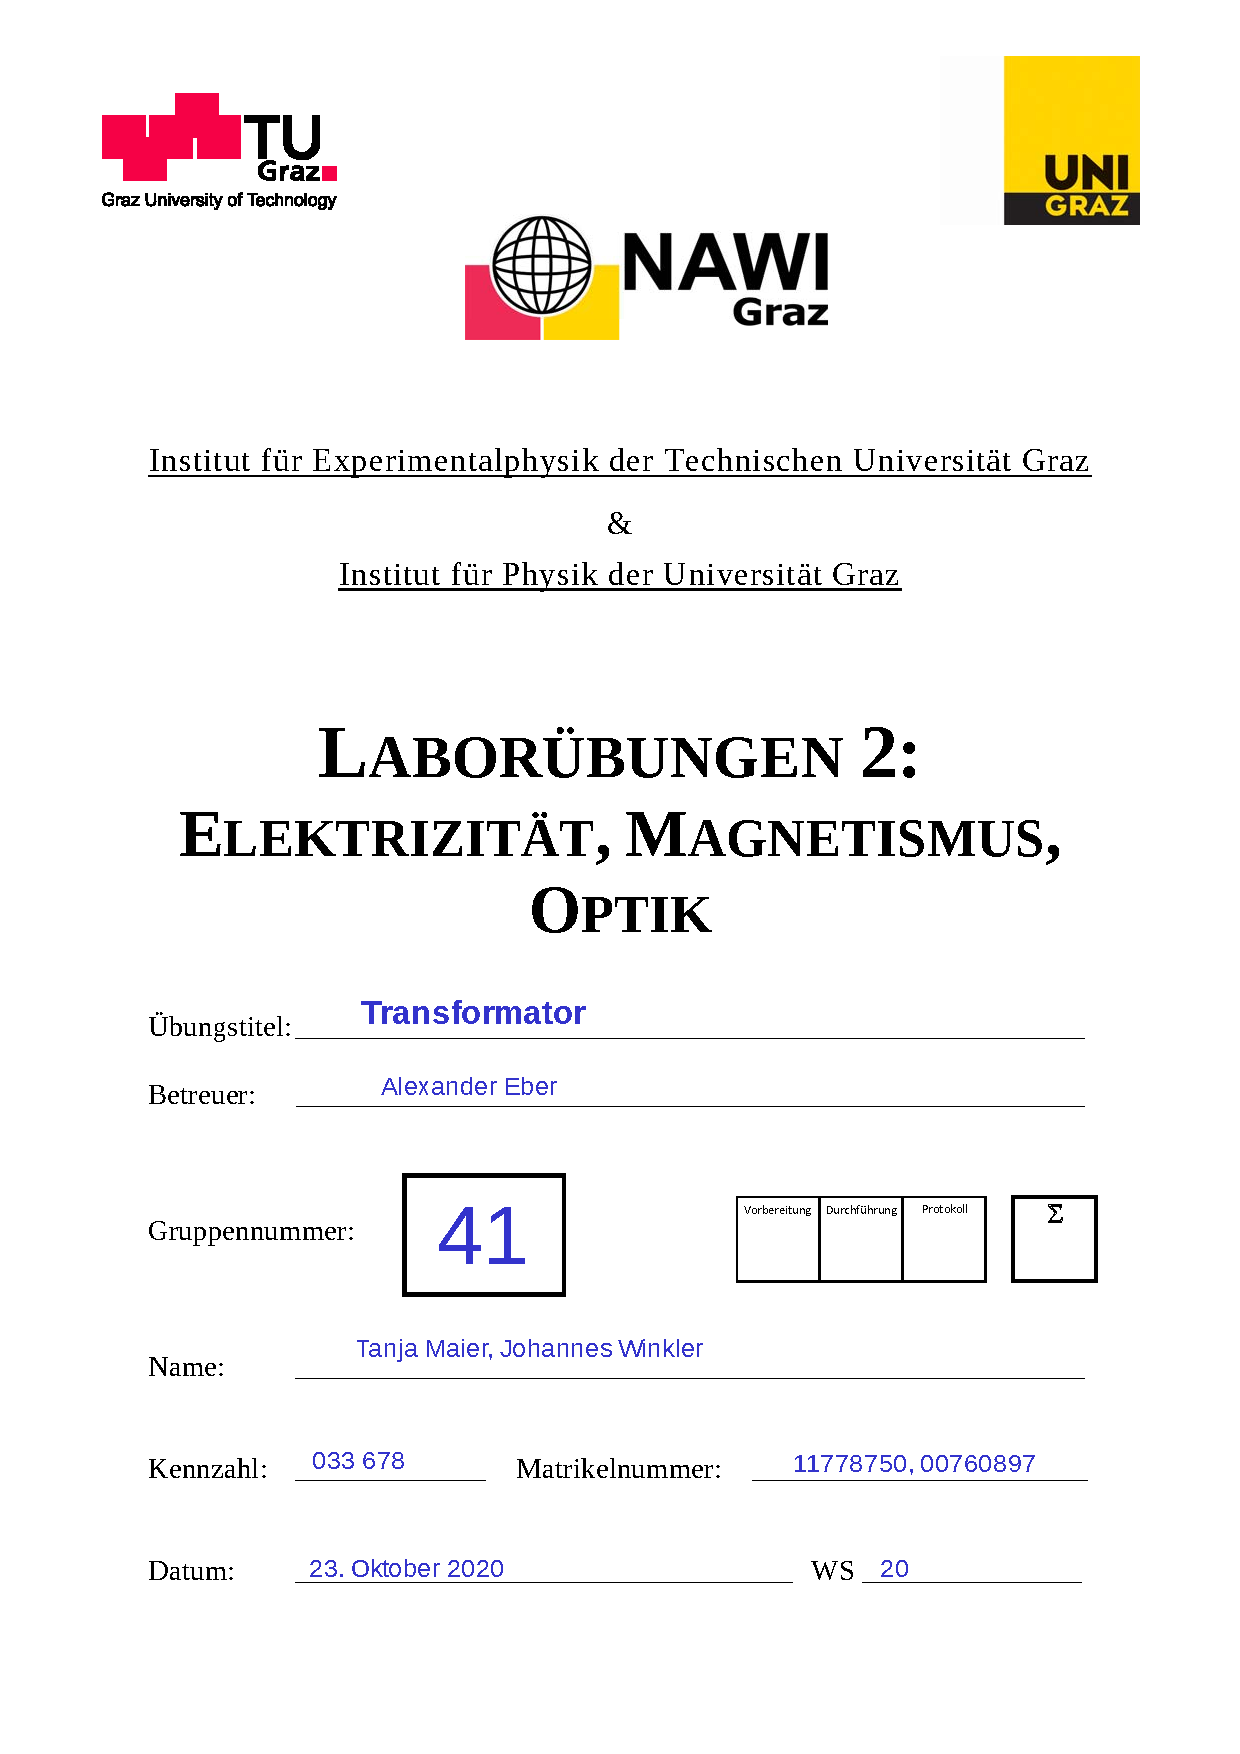
\includepdf{Deckblatt.pdf}


\pagestyle{fancy}

\section{Aufgabenstellung}






\section{Grundlagen und Versuchsaufbau}




\begin{figure}[H]
\caption{Ionentransport im Elektrolyten im elektrischen Feld. $A$ Anode, $K$ Kathode.}
\label{fig:pic1}
{\centering
%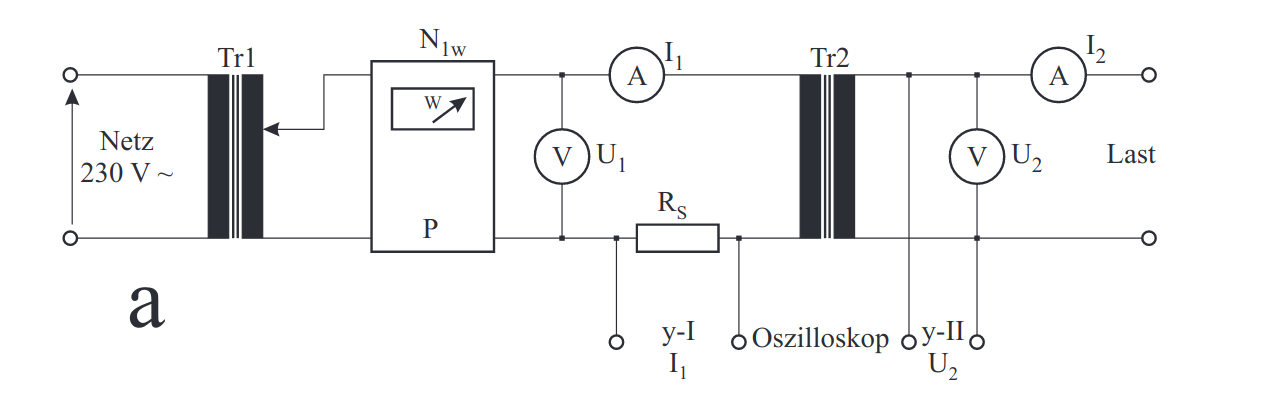
\includegraphics[scale=1.8]{pic1.png}
~
}
\end{figure}



\section{Geräteliste}

\begin{table}[H]
\caption{Liste der verwendeten Geräte}

~

\begin{tabular}{l|llll}
Bezeichnung & Hersteller & Gerätenummer & Unsicherheit \\
\hline
Thermometer & & & $\pm 1~^\circ$C \\
Frequenzgenerator & Wavetek & 0161674  \\
Trenntransformator & \\
Oszilloskop & RIGOL &DS1ET204711289 \\
Widerstand $1$~k$\Omega$ & Rosenthal & & $\pm~1\%$ \\
Widerstand $200~\Omega$ & Rosenthal & & $\pm~1\%$ \\
2x Spule $n=500$ & & 843/3 \\
Kondensator $1~\mu$F & Philips
\end{tabular}

\end{table}




\section{Durchführung und Messwerte}



\section{Auswertung}



\section{Zusammenfassung}




\section{Diskussion}





%\newpage 
%\appendix
%\section{Python Skript}



\definecolor{commentgreen}{RGB}{2,112,10}
\definecolor{eminence}{RGB}{108,48,130}
\definecolor{weborange}{RGB}{255,165,0}
\definecolor{frenchplum}{RGB}{129,20,83}

\lstdefinelanguage{python}{
    morekeywords={def, for, range, abs, return},
    otherkeywords={<-,->, |>, \%\{, \}, \{, \, (, )},
    sensitive=true,
    morecomment=[l]{\#},
    morecomment=[n]{/*}{*/},
    morecomment=[s][\color{purple}]{:}{\ },
    morestring=[s][\color{orange}]"",
    commentstyle=\color{commentgreen},
    keywordstyle=\color{eminence},
    stringstyle=\color{red},
	basicstyle=\ttfamily,
	breaklines,
	showstringspaces=false,
	frame=tb
}
%\lstinputlisting[language=Python,captionpos=b, label=lst:test,caption={Sinus Auswertung von Schaltung 1}]{analyse/analyse_ges.py}

%\lstinputlisting[language=Python,captionpos=b, label=lst:test,caption={Bessel Auswertung}]{generate_numbers_bessel.py}


%\lstinputlisting[language=Python,captionpos=b, label=lst:test,caption={Zerstreuungslinse Auswertung}]{generate_numbers_zerstreuungslinse.py}


\begin{thebibliography}{9}
\bibitem{chemie} \url{https://www.chemie.de/lexikon/Elektrochemisches_äquivalent.html}, 22.10.2020 22:53 Uhr
\bibitem{tu} bereitgestellte Unterlagen zum Versuch aus dem TeachCenter der TU Graz
\end{thebibliography}


\end{document}
